% =====================================================================
% figE  — R/ggplot2 -> tikzDevice (parallel to ../figures-tex/figE_deletion.tex)
% Canonical-JSON-only. Regenerate: Rscript figures-r/make_figures.R
% Provenance (JSON path :: field = plotted value), one line per series:
% SOURCE: results/C3_u1_blockB_L8_seeds_u5.json :: aggregate.within_probe_mean_across_seeds = 0.4610
% SOURCE: results/U1_E1_transplant_GATE_L12_s{0,1,2}.json :: mean(keycos.within_probe_mean) = 0.6626
% SOURCE: results/C3_u1_blockB_L14_seeds_u5.json :: aggregate.within_probe_mean_across_seeds = 0.5191
% SOURCE: results/G1_L12_analysis.json :: aggregate.within_probe_mean_across_seeds (rewrite ref) = 0.6018
% SOURCE: results/u1_gate_refusal_L12_s0.json :: arms['known=True|edit_ok=False'].nondc_rho = 0.6571
% SOURCE: results/u1_gate_refusal_L12_s0.json :: arms['known=True|edit_ok=False'].dc_rho = 0.4371
% SOURCE: results/u1_gate_eos_L12_s0.json :: arms['known=True|edit_ok=False'].nondc_rho = 0.6530
% SOURCE: results/u1_gate_eos_L12_s0.json :: arms['known=True|edit_ok=False'].dc_rho = 0.4823
% SOURCE: results/u1_gate_suppress_L12_s0.json :: arms['known=True|edit_ok=False'].nondc_rho = 0.6213
% SOURCE: results/u1_gate_suppress_L12_s0.json :: arms['known=True|edit_ok=False'].dc_rho = 0.1587
% SOURCE: results/U1_E1_transplant_GATE_L12_s{0,1,2}.json :: mean(mean_signed_damage) = 3.7888
% SOURCE: results/U1_E1_transplant_GATE_L12_s{0,1,2}.json :: mean(SxC_within_probe_mean) = 0.6779
% SOURCE: results/U1_E1_transplant_GATE_alphadelete_L12_s{0,1,2}.json :: mean(mean_signed_damage) = 0.1055
% SOURCE: results/C3_u1_blockD_alphadelete_seeds_u2.json :: aggregate.within_probe_mean_across_seeds = 0.0362
% SOURCE: results/U1_E1_transplant_GATE_L8_s0.json :: delta_rho_SxC_minus_best_transplant = 0.3140
% SOURCE: results/U1_E1_transplant_GATE_L12_s0.json :: delta_rho_SxC_minus_best_transplant = 0.5935
% SOURCE: results/U1_E1_transplant_GATE_L12_s1.json :: delta_rho_SxC_minus_best_transplant = 0.5458
% SOURCE: results/U1_E1_transplant_GATE_L12_s2.json :: delta_rho_SxC_minus_best_transplant = 0.6124
% SOURCE: results/U1_E1_transplant_GATE_L14_s0.json :: delta_rho_SxC_minus_best_transplant = 0.3838
% =====================================================================
% !TEX encoding = UTF-8 Unicode
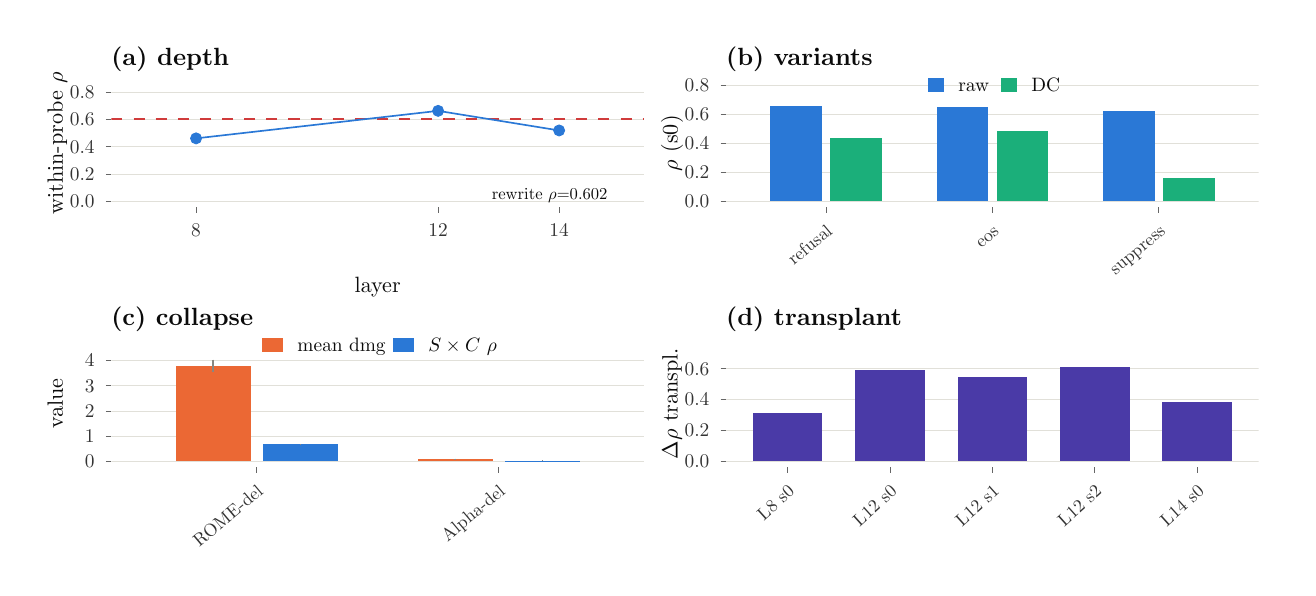
\begin{tikzpicture}[x=1pt,y=1pt]
\definecolor{fillColor}{RGB}{255,255,255}
\path[use as bounding box,fill=fillColor,fill opacity=0.00] (0,0) rectangle (455.30,195.13);
\begin{scope}
\path[clip] (  0.00,  0.00) rectangle (455.30,195.13);
\definecolor{drawColor}{RGB}{255,255,255}
\definecolor{fillColor}{RGB}{255,255,255}

\path[draw=drawColor,line width= 0.6pt,line join=round,line cap=round,fill=fillColor] (  0.00,  0.00) rectangle (455.30,195.13);
\end{scope}
\begin{scope}
\path[clip] (  5.50, 95.60) rectangle (227.65,189.63);
\definecolor{fillColor}{RGB}{255,255,255}

\path[fill=fillColor] (  5.50, 95.60) rectangle (227.65,189.63);
\end{scope}
\begin{scope}
\path[clip] (227.65, 95.60) rectangle (449.80,189.63);
\definecolor{fillColor}{RGB}{255,255,255}

\path[fill=fillColor] (227.65, 95.60) rectangle (449.80,189.63);
\end{scope}
\begin{scope}
\path[clip] ( 30.24,130.30) rectangle (222.65,176.41);
\definecolor{drawColor}{RGB}{225,224,217}

\path[draw=drawColor,line width= 0.3pt,line join=round] ( 30.24,132.39) --
	(222.65,132.39);

\path[draw=drawColor,line width= 0.3pt,line join=round] ( 30.24,142.26) --
	(222.65,142.26);

\path[draw=drawColor,line width= 0.3pt,line join=round] ( 30.24,152.12) --
	(222.65,152.12);

\path[draw=drawColor,line width= 0.3pt,line join=round] ( 30.24,161.98) --
	(222.65,161.98);

\path[draw=drawColor,line width= 0.3pt,line join=round] ( 30.24,171.85) --
	(222.65,171.85);
\definecolor{drawColor}{RGB}{208,59,59}

\path[draw=drawColor,line width= 0.5pt,dash pattern=on 4pt off 4pt ,line join=round] ( 30.24,162.07) -- (222.65,162.07);
\definecolor{drawColor}{RGB}{11,11,11}

\node[text=drawColor,anchor=base east,inner sep=0pt, outer sep=0pt, scale=  0.60] at (209.53,132.92) {rewrite $\rho{=}0.602$};
\definecolor{drawColor}{RGB}{137,135,129}

\path[draw=drawColor,line width= 0.4pt,line join=round] ( 60.85,155.97) --
	( 60.85,155.97);

\path[draw=drawColor,line width= 0.4pt,line join=round] ( 60.85,155.97) --
	( 60.85,154.29);

\path[draw=drawColor,line width= 0.4pt,line join=round] ( 60.85,154.29) --
	( 60.85,154.29);

\path[draw=drawColor,line width= 0.4pt,line join=round] (148.31,165.98) --
	(148.31,165.98);

\path[draw=drawColor,line width= 0.4pt,line join=round] (148.31,165.98) --
	(148.31,164.16);

\path[draw=drawColor,line width= 0.4pt,line join=round] (148.31,164.16) --
	(148.31,164.16);

\path[draw=drawColor,line width= 0.4pt,line join=round] (192.04,158.86) --
	(192.04,158.86);

\path[draw=drawColor,line width= 0.4pt,line join=round] (192.04,158.86) --
	(192.04,157.13);

\path[draw=drawColor,line width= 0.4pt,line join=round] (192.04,157.13) --
	(192.04,157.13);
\definecolor{drawColor}{RGB}{42,120,214}

\path[draw=drawColor,line width= 0.6pt,line join=round] ( 60.85,155.13) --
	(148.31,165.07) --
	(192.04,157.99);
\definecolor{fillColor}{RGB}{42,120,214}

\path[draw=drawColor,line width= 0.3pt,line join=round,line cap=round,fill=fillColor] ( 60.85,155.13) circle (  2.00);

\path[draw=drawColor,line width= 0.3pt,line join=round,line cap=round,fill=fillColor] (148.31,165.07) circle (  2.00);

\path[draw=drawColor,line width= 0.3pt,line join=round,line cap=round,fill=fillColor] (192.04,157.99) circle (  2.00);
\end{scope}
\begin{scope}
\path[clip] (  0.00,  0.00) rectangle (455.30,195.13);
\definecolor{drawColor}{gray}{0.20}

\node[text=drawColor,anchor=base east,inner sep=0pt, outer sep=0pt, scale=  0.70] at ( 24.19,130.12) {0.0};

\node[text=drawColor,anchor=base east,inner sep=0pt, outer sep=0pt, scale=  0.70] at ( 24.19,139.98) {0.2};

\node[text=drawColor,anchor=base east,inner sep=0pt, outer sep=0pt, scale=  0.70] at ( 24.19,149.84) {0.4};

\node[text=drawColor,anchor=base east,inner sep=0pt, outer sep=0pt, scale=  0.70] at ( 24.19,159.70) {0.6};

\node[text=drawColor,anchor=base east,inner sep=0pt, outer sep=0pt, scale=  0.70] at ( 24.19,169.57) {0.8};
\end{scope}
\begin{scope}
\path[clip] (  0.00,  0.00) rectangle (455.30,195.13);
\definecolor{drawColor}{gray}{0.40}

\path[draw=drawColor,line width= 0.3pt,line join=round] ( 28.24,132.39) --
	( 30.24,132.39);

\path[draw=drawColor,line width= 0.3pt,line join=round] ( 28.24,142.26) --
	( 30.24,142.26);

\path[draw=drawColor,line width= 0.3pt,line join=round] ( 28.24,152.12) --
	( 30.24,152.12);

\path[draw=drawColor,line width= 0.3pt,line join=round] ( 28.24,161.98) --
	( 30.24,161.98);

\path[draw=drawColor,line width= 0.3pt,line join=round] ( 28.24,171.85) --
	( 30.24,171.85);
\end{scope}
\begin{scope}
\path[clip] (  0.00,  0.00) rectangle (455.30,195.13);
\definecolor{drawColor}{gray}{0.40}

\path[draw=drawColor,line width= 0.3pt,line join=round] ( 60.85,128.30) --
	( 60.85,130.30);

\path[draw=drawColor,line width= 0.3pt,line join=round] (148.31,128.30) --
	(148.31,130.30);

\path[draw=drawColor,line width= 0.3pt,line join=round] (192.04,128.30) --
	(192.04,130.30);
\end{scope}
\begin{scope}
\path[clip] (  0.00,  0.00) rectangle (455.30,195.13);
\definecolor{drawColor}{gray}{0.20}

\node[text=drawColor,anchor=base,inner sep=0pt, outer sep=0pt, scale=  0.70] at ( 60.85,119.69) {8};

\node[text=drawColor,anchor=base,inner sep=0pt, outer sep=0pt, scale=  0.70] at (148.31,119.69) {12};

\node[text=drawColor,anchor=base,inner sep=0pt, outer sep=0pt, scale=  0.70] at (192.04,119.69) {14};
\end{scope}
\begin{scope}
\path[clip] (  0.00,  0.00) rectangle (455.30,195.13);
\definecolor{drawColor}{RGB}{11,11,11}

\node[text=drawColor,anchor=base,inner sep=0pt, outer sep=0pt, scale=  0.80] at (126.45, 99.33) {layer};
\end{scope}
\begin{scope}
\path[clip] (  0.00,  0.00) rectangle (455.30,195.13);
\definecolor{drawColor}{RGB}{11,11,11}

\node[text=drawColor,rotate= 90.00,anchor=base,inner sep=0pt, outer sep=0pt, scale=  0.80] at ( 12.71,153.35) {within-probe $\rho$};
\end{scope}
\begin{scope}
\path[clip] (  0.00,  0.00) rectangle (455.30,195.13);
\definecolor{drawColor}{RGB}{11,11,11}

\node[text=drawColor,anchor=base west,inner sep=0pt, outer sep=0pt, scale=  0.90] at ( 30.24,181.43) {\bfseries (a) depth};
\end{scope}
\begin{scope}
\path[clip] (252.39,130.30) rectangle (444.80,176.41);
\definecolor{drawColor}{RGB}{225,224,217}

\path[draw=drawColor,line width= 0.3pt,line join=round] (252.39,132.39) --
	(444.80,132.39);

\path[draw=drawColor,line width= 0.3pt,line join=round] (252.39,142.87) --
	(444.80,142.87);

\path[draw=drawColor,line width= 0.3pt,line join=round] (252.39,153.35) --
	(444.80,153.35);

\path[draw=drawColor,line width= 0.3pt,line join=round] (252.39,163.83) --
	(444.80,163.83);

\path[draw=drawColor,line width= 0.3pt,line join=round] (252.39,174.31) --
	(444.80,174.31);
\definecolor{fillColor}{RGB}{42,120,214}

\path[fill=fillColor] (268.32,132.39) rectangle (286.96,166.82);
\definecolor{fillColor}{RGB}{27,175,122}

\path[fill=fillColor] (289.97,132.39) rectangle (308.61,155.30);
\definecolor{fillColor}{RGB}{42,120,214}

\path[fill=fillColor] (328.45,132.39) rectangle (347.09,166.61);
\definecolor{fillColor}{RGB}{27,175,122}

\path[fill=fillColor] (350.10,132.39) rectangle (368.74,157.67);
\definecolor{fillColor}{RGB}{42,120,214}

\path[fill=fillColor] (388.58,132.39) rectangle (407.22,164.95);
\definecolor{fillColor}{RGB}{27,175,122}

\path[fill=fillColor] (410.23,132.39) rectangle (428.87,140.71);
\end{scope}
\begin{scope}
\path[clip] (  0.00,  0.00) rectangle (455.30,195.13);
\definecolor{drawColor}{gray}{0.20}

\node[text=drawColor,anchor=base east,inner sep=0pt, outer sep=0pt, scale=  0.70] at (246.34,130.12) {0.0};

\node[text=drawColor,anchor=base east,inner sep=0pt, outer sep=0pt, scale=  0.70] at (246.34,140.60) {0.2};

\node[text=drawColor,anchor=base east,inner sep=0pt, outer sep=0pt, scale=  0.70] at (246.34,151.07) {0.4};

\node[text=drawColor,anchor=base east,inner sep=0pt, outer sep=0pt, scale=  0.70] at (246.34,161.55) {0.6};

\node[text=drawColor,anchor=base east,inner sep=0pt, outer sep=0pt, scale=  0.70] at (246.34,172.03) {0.8};
\end{scope}
\begin{scope}
\path[clip] (  0.00,  0.00) rectangle (455.30,195.13);
\definecolor{drawColor}{gray}{0.40}

\path[draw=drawColor,line width= 0.3pt,line join=round] (250.39,132.39) --
	(252.39,132.39);

\path[draw=drawColor,line width= 0.3pt,line join=round] (250.39,142.87) --
	(252.39,142.87);

\path[draw=drawColor,line width= 0.3pt,line join=round] (250.39,153.35) --
	(252.39,153.35);

\path[draw=drawColor,line width= 0.3pt,line join=round] (250.39,163.83) --
	(252.39,163.83);

\path[draw=drawColor,line width= 0.3pt,line join=round] (250.39,174.31) --
	(252.39,174.31);
\end{scope}
\begin{scope}
\path[clip] (  0.00,  0.00) rectangle (455.30,195.13);
\definecolor{drawColor}{gray}{0.40}

\path[draw=drawColor,line width= 0.3pt,line join=round] (288.47,128.30) --
	(288.47,130.30);

\path[draw=drawColor,line width= 0.3pt,line join=round] (348.60,128.30) --
	(348.60,130.30);

\path[draw=drawColor,line width= 0.3pt,line join=round] (408.72,128.30) --
	(408.72,130.30);
\end{scope}
\begin{scope}
\path[clip] (  0.00,  0.00) rectangle (455.30,195.13);
\definecolor{drawColor}{gray}{0.20}

\node[text=drawColor,rotate= 40.00,anchor=base east,inner sep=0pt, outer sep=0pt, scale=  0.65] at (291.19,121.01) {refusal};

\node[text=drawColor,rotate= 40.00,anchor=base east,inner sep=0pt, outer sep=0pt, scale=  0.65] at (351.32,121.01) {eos};

\node[text=drawColor,rotate= 40.00,anchor=base east,inner sep=0pt, outer sep=0pt, scale=  0.65] at (411.44,121.01) {suppress};
\end{scope}
\begin{scope}
\path[clip] (  0.00,  0.00) rectangle (455.30,195.13);
\definecolor{drawColor}{RGB}{11,11,11}

\node[text=drawColor,rotate= 90.00,anchor=base,inner sep=0pt, outer sep=0pt, scale=  0.80] at (234.86,153.35) {$\rho$ (s0)};
\end{scope}
\begin{scope}
\path[clip] (  0.00,  0.00) rectangle (455.30,195.13);
\definecolor{fillColor}{RGB}{42,120,214}

\path[fill=fillColor] (325.37,171.99) rectangle (331.21,176.90);
\end{scope}
\begin{scope}
\path[clip] (  0.00,  0.00) rectangle (455.30,195.13);
\definecolor{fillColor}{RGB}{27,175,122}

\path[fill=fillColor] (351.76,171.99) rectangle (357.60,176.90);
\end{scope}
\begin{scope}
\path[clip] (  0.00,  0.00) rectangle (455.30,195.13);
\definecolor{drawColor}{RGB}{11,11,11}

\node[text=drawColor,anchor=base west,inner sep=0pt, outer sep=0pt, scale=  0.70] at (336.29,172.17) {raw};
\end{scope}
\begin{scope}
\path[clip] (  0.00,  0.00) rectangle (455.30,195.13);
\definecolor{drawColor}{RGB}{11,11,11}

\node[text=drawColor,anchor=base west,inner sep=0pt, outer sep=0pt, scale=  0.70] at (362.68,172.17) {DC};
\end{scope}
\begin{scope}
\path[clip] (  0.00,  0.00) rectangle (455.30,195.13);
\definecolor{drawColor}{RGB}{11,11,11}

\node[text=drawColor,anchor=base west,inner sep=0pt, outer sep=0pt, scale=  0.90] at (252.39,181.43) {\bfseries (b) variants};
\end{scope}
\begin{scope}
\path[clip] (  5.50,  5.50) rectangle (227.65, 95.60);
\definecolor{fillColor}{RGB}{255,255,255}

\path[fill=fillColor] (  5.50,  5.50) rectangle (227.65, 95.60);
\end{scope}
\begin{scope}
\path[clip] (227.65,  5.50) rectangle (449.80, 95.60);
\definecolor{fillColor}{RGB}{255,255,255}

\path[fill=fillColor] (227.65,  5.50) rectangle (449.80, 95.60);
\end{scope}
\begin{scope}
\path[clip] ( 30.24, 36.27) rectangle (222.65, 82.38);
\definecolor{drawColor}{RGB}{225,224,217}

\path[draw=drawColor,line width= 0.3pt,line join=round] ( 30.24, 38.37) --
	(222.65, 38.37);

\path[draw=drawColor,line width= 0.3pt,line join=round] ( 30.24, 47.48) --
	(222.65, 47.48);

\path[draw=drawColor,line width= 0.3pt,line join=round] ( 30.24, 56.59) --
	(222.65, 56.59);

\path[draw=drawColor,line width= 0.3pt,line join=round] ( 30.24, 65.70) --
	(222.65, 65.70);

\path[draw=drawColor,line width= 0.3pt,line join=round] ( 30.24, 74.82) --
	(222.65, 74.82);
\definecolor{fillColor}{RGB}{235,104,52}

\path[fill=fillColor] ( 53.42, 38.37) rectangle ( 80.53, 72.89);

\path[fill=fillColor] (140.88, 38.37) rectangle (167.99, 39.33);
\definecolor{fillColor}{RGB}{42,120,214}

\path[fill=fillColor] ( 84.90, 38.37) rectangle (112.01, 44.54);

\path[fill=fillColor] (172.36, 38.37) rectangle (199.47, 38.70);
\definecolor{drawColor}{RGB}{137,135,129}

\path[draw=drawColor,line width= 0.4pt,line join=round] ( 66.97, 75.21) --
	( 66.97, 75.21);

\path[draw=drawColor,line width= 0.4pt,line join=round] ( 66.97, 75.21) --
	( 66.97, 70.57);

\path[draw=drawColor,line width= 0.4pt,line join=round] ( 66.97, 70.57) --
	( 66.97, 70.57);

\path[draw=drawColor,line width= 0.4pt,line join=round] (154.43, 39.36) --
	(154.43, 39.36);

\path[draw=drawColor,line width= 0.4pt,line join=round] (154.43, 39.36) --
	(154.43, 39.29);

\path[draw=drawColor,line width= 0.4pt,line join=round] (154.43, 39.29) --
	(154.43, 39.29);

\path[draw=drawColor,line width= 0.4pt,line join=round] ( 98.46, 44.69) --
	( 98.46, 44.69);

\path[draw=drawColor,line width= 0.4pt,line join=round] ( 98.46, 44.69) --
	( 98.46, 44.40);

\path[draw=drawColor,line width= 0.4pt,line join=round] ( 98.46, 44.40) --
	( 98.46, 44.40);

\path[draw=drawColor,line width= 0.4pt,line join=round] (185.92, 38.83) --
	(185.92, 38.83);

\path[draw=drawColor,line width= 0.4pt,line join=round] (185.92, 38.83) --
	(185.92, 38.56);

\path[draw=drawColor,line width= 0.4pt,line join=round] (185.92, 38.56) --
	(185.92, 38.56);
\end{scope}
\begin{scope}
\path[clip] (  0.00,  0.00) rectangle (455.30,195.13);
\definecolor{drawColor}{gray}{0.20}

\node[text=drawColor,anchor=base east,inner sep=0pt, outer sep=0pt, scale=  0.70] at ( 24.19, 36.09) {0};

\node[text=drawColor,anchor=base east,inner sep=0pt, outer sep=0pt, scale=  0.70] at ( 24.19, 45.20) {1};

\node[text=drawColor,anchor=base east,inner sep=0pt, outer sep=0pt, scale=  0.70] at ( 24.19, 54.31) {2};

\node[text=drawColor,anchor=base east,inner sep=0pt, outer sep=0pt, scale=  0.70] at ( 24.19, 63.42) {3};

\node[text=drawColor,anchor=base east,inner sep=0pt, outer sep=0pt, scale=  0.70] at ( 24.19, 72.54) {4};
\end{scope}
\begin{scope}
\path[clip] (  0.00,  0.00) rectangle (455.30,195.13);
\definecolor{drawColor}{gray}{0.40}

\path[draw=drawColor,line width= 0.3pt,line join=round] ( 28.24, 38.37) --
	( 30.24, 38.37);

\path[draw=drawColor,line width= 0.3pt,line join=round] ( 28.24, 47.48) --
	( 30.24, 47.48);

\path[draw=drawColor,line width= 0.3pt,line join=round] ( 28.24, 56.59) --
	( 30.24, 56.59);

\path[draw=drawColor,line width= 0.3pt,line join=round] ( 28.24, 65.70) --
	( 30.24, 65.70);

\path[draw=drawColor,line width= 0.3pt,line join=round] ( 28.24, 74.82) --
	( 30.24, 74.82);
\end{scope}
\begin{scope}
\path[clip] (  0.00,  0.00) rectangle (455.30,195.13);
\definecolor{drawColor}{gray}{0.40}

\path[draw=drawColor,line width= 0.3pt,line join=round] ( 82.72, 34.27) --
	( 82.72, 36.27);

\path[draw=drawColor,line width= 0.3pt,line join=round] (170.17, 34.27) --
	(170.17, 36.27);
\end{scope}
\begin{scope}
\path[clip] (  0.00,  0.00) rectangle (455.30,195.13);
\definecolor{drawColor}{gray}{0.20}

\node[text=drawColor,rotate= 40.00,anchor=base east,inner sep=0pt, outer sep=0pt, scale=  0.65] at ( 85.44, 26.98) {ROME-del};

\node[text=drawColor,rotate= 40.00,anchor=base east,inner sep=0pt, outer sep=0pt, scale=  0.65] at (172.89, 26.98) {Alpha-del};
\end{scope}
\begin{scope}
\path[clip] (  0.00,  0.00) rectangle (455.30,195.13);
\definecolor{drawColor}{RGB}{11,11,11}

\node[text=drawColor,rotate= 90.00,anchor=base,inner sep=0pt, outer sep=0pt, scale=  0.80] at ( 12.71, 59.32) {value};
\end{scope}
\begin{scope}
\path[clip] (  0.00,  0.00) rectangle (455.30,195.13);
\definecolor{fillColor}{RGB}{235,104,52}

\path[fill=fillColor] ( 84.54, 77.96) rectangle ( 92.37, 82.87);
\end{scope}
\begin{scope}
\path[clip] (  0.00,  0.00) rectangle (455.30,195.13);
\definecolor{fillColor}{RGB}{42,120,214}

\path[fill=fillColor] (131.89, 77.96) rectangle (139.73, 82.87);
\end{scope}
\begin{scope}
\path[clip] (  0.00,  0.00) rectangle (455.30,195.13);
\definecolor{drawColor}{RGB}{11,11,11}

\node[text=drawColor,anchor=base west,inner sep=0pt, outer sep=0pt, scale=  0.70] at ( 97.45, 78.14) {mean dmg};
\end{scope}
\begin{scope}
\path[clip] (  0.00,  0.00) rectangle (455.30,195.13);
\definecolor{drawColor}{RGB}{11,11,11}

\node[text=drawColor,anchor=base west,inner sep=0pt, outer sep=0pt, scale=  0.70] at (144.81, 78.14) {$S\times C$ $\rho$};
\end{scope}
\begin{scope}
\path[clip] (  0.00,  0.00) rectangle (455.30,195.13);
\definecolor{drawColor}{RGB}{11,11,11}

\node[text=drawColor,anchor=base west,inner sep=0pt, outer sep=0pt, scale=  0.90] at ( 30.24, 87.40) {\bfseries (c) collapse};
\end{scope}
\begin{scope}
\path[clip] (252.39, 36.27) rectangle (444.80, 82.38);
\definecolor{drawColor}{RGB}{225,224,217}

\path[draw=drawColor,line width= 0.3pt,line join=round] (252.39, 38.37) --
	(444.80, 38.37);

\path[draw=drawColor,line width= 0.3pt,line join=round] (252.39, 49.54) --
	(444.80, 49.54);

\path[draw=drawColor,line width= 0.3pt,line join=round] (252.39, 60.72) --
	(444.80, 60.72);

\path[draw=drawColor,line width= 0.3pt,line join=round] (252.39, 71.90) --
	(444.80, 71.90);
\definecolor{fillColor}{RGB}{74,58,167}

\path[fill=fillColor] (262.01, 38.37) rectangle (287.17, 55.91);

\path[fill=fillColor] (299.01, 38.37) rectangle (324.17, 71.54);

\path[fill=fillColor] (336.01, 38.37) rectangle (361.18, 68.87);

\path[fill=fillColor] (373.02, 38.37) rectangle (398.18, 72.59);

\path[fill=fillColor] (410.02, 38.37) rectangle (435.18, 59.82);
\end{scope}
\begin{scope}
\path[clip] (  0.00,  0.00) rectangle (455.30,195.13);
\definecolor{drawColor}{gray}{0.20}

\node[text=drawColor,anchor=base east,inner sep=0pt, outer sep=0pt, scale=  0.70] at (246.34, 36.09) {0.0};

\node[text=drawColor,anchor=base east,inner sep=0pt, outer sep=0pt, scale=  0.70] at (246.34, 47.26) {0.2};

\node[text=drawColor,anchor=base east,inner sep=0pt, outer sep=0pt, scale=  0.70] at (246.34, 58.44) {0.4};

\node[text=drawColor,anchor=base east,inner sep=0pt, outer sep=0pt, scale=  0.70] at (246.34, 69.62) {0.6};
\end{scope}
\begin{scope}
\path[clip] (  0.00,  0.00) rectangle (455.30,195.13);
\definecolor{drawColor}{gray}{0.40}

\path[draw=drawColor,line width= 0.3pt,line join=round] (250.39, 38.37) --
	(252.39, 38.37);

\path[draw=drawColor,line width= 0.3pt,line join=round] (250.39, 49.54) --
	(252.39, 49.54);

\path[draw=drawColor,line width= 0.3pt,line join=round] (250.39, 60.72) --
	(252.39, 60.72);

\path[draw=drawColor,line width= 0.3pt,line join=round] (250.39, 71.90) --
	(252.39, 71.90);
\end{scope}
\begin{scope}
\path[clip] (  0.00,  0.00) rectangle (455.30,195.13);
\definecolor{drawColor}{gray}{0.40}

\path[draw=drawColor,line width= 0.3pt,line join=round] (274.59, 34.27) --
	(274.59, 36.27);

\path[draw=drawColor,line width= 0.3pt,line join=round] (311.59, 34.27) --
	(311.59, 36.27);

\path[draw=drawColor,line width= 0.3pt,line join=round] (348.60, 34.27) --
	(348.60, 36.27);

\path[draw=drawColor,line width= 0.3pt,line join=round] (385.60, 34.27) --
	(385.60, 36.27);

\path[draw=drawColor,line width= 0.3pt,line join=round] (422.60, 34.27) --
	(422.60, 36.27);
\end{scope}
\begin{scope}
\path[clip] (  0.00,  0.00) rectangle (455.30,195.13);
\definecolor{drawColor}{gray}{0.20}

\node[text=drawColor,rotate= 42.00,anchor=base east,inner sep=0pt, outer sep=0pt, scale=  0.65] at (277.42, 27.07) {L8 s0};

\node[text=drawColor,rotate= 42.00,anchor=base east,inner sep=0pt, outer sep=0pt, scale=  0.65] at (314.42, 27.07) {L12 s0};

\node[text=drawColor,rotate= 42.00,anchor=base east,inner sep=0pt, outer sep=0pt, scale=  0.65] at (351.43, 27.07) {L12 s1};

\node[text=drawColor,rotate= 42.00,anchor=base east,inner sep=0pt, outer sep=0pt, scale=  0.65] at (388.43, 27.07) {L12 s2};

\node[text=drawColor,rotate= 42.00,anchor=base east,inner sep=0pt, outer sep=0pt, scale=  0.65] at (425.43, 27.07) {L14 s0};
\end{scope}
\begin{scope}
\path[clip] (  0.00,  0.00) rectangle (455.30,195.13);
\definecolor{drawColor}{RGB}{11,11,11}

\node[text=drawColor,rotate= 90.00,anchor=base,inner sep=0pt, outer sep=0pt, scale=  0.80] at (234.86, 59.32) {$\Delta\rho$ transpl.};
\end{scope}
\begin{scope}
\path[clip] (  0.00,  0.00) rectangle (455.30,195.13);
\definecolor{drawColor}{RGB}{11,11,11}

\node[text=drawColor,anchor=base west,inner sep=0pt, outer sep=0pt, scale=  0.90] at (252.39, 87.40) {\bfseries (d) transplant};
\end{scope}
\end{tikzpicture}
